\documentclass[a4paper]{article}
\usepackage[pdftex]{graphicx}
\usepackage[utf8]{inputenc}
\usepackage{enumerate}
\usepackage{siunitx}
\sisetup{locale=DE} 
\usepackage{icomma}
\usepackage{amssymb}
\usepackage{eurosym}
\usepackage{tikz}
\usepackage{href-ul}
\hypersetup{
	colorlinks=true,
	linkcolor=blue,
	urlcolor=blue}
\usepackage{geometry}
\geometry{a4paper, top=15mm, left=15mm, right=15mm, bottom=15mm,
	headsep=10mm, footskip=12mm}

\begin{document}
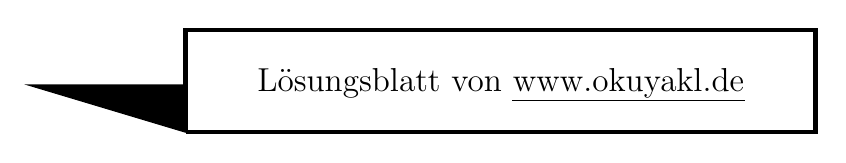
\begin{tikzpicture}(10,3)
	\draw[ultra thick](2,0) --(10,0) -- (10,1.3) --(2,1.3) -- (2,0);
	\draw[fill=black](2,0)-- (0,.6) -- (2,.6) -- (2,0);
	\node at (6,.6) {\large Lösungsblatt von \href{https://www.okuyakl.de}{www.okuyakl.de}};
\end{tikzpicture}
\vspace{0.5 cm}


\noindent{\bf Aufgabe 1. a)}\\
Wir nehmen eine Metallplatte mit einem kreisrunden Loch, durch welches eine Stahlkugel gerade so durchpasst. Nun erhitzen wir die Kugel mit einem Bunsenbrenner und stellen fest, dass sie nun nicht mehr hindurchpasst.
\vspace{0.5 cm}

\noindent{\bf Aufgabe 1. b)}\\ 
In einem Feststoff liegen die Atome dicht an dicht angeordnet. Bei Erwärmung schwingen diese nun stärker um ihre Ruhelage. Durch stärkere Stöße mit Nachbaratomen vergrößert sich der Abstand. Dadurch gewinnen sie neben kinetischer Energie auch potentielle. Beide setzen sich zusammen zu innerer Energie.
\vspace{0.5 cm}

\noindent{\bf Aufgabe 1. c)}\\
Zunächst berechnen wir den Längenausdehnungskoeffizient $\alpha$ von Stahl:
$$\alpha = {\Delta l \over l \cdot T} = {\SI{12e-6}{\meter}\over \SI{1}{\meter}\cdot \SI{1}{\kelvin}}=
\SI{12e-6}{\kelvin^{-1}}$$
Die Längenänderung der Schiene ist dann:
$$\Delta l_s = l_s \cdot \alpha \cdot \Delta \vartheta = \SI{30}{\meter} \cdot \SI{12e-6}{\kelvin^{-1}}\cdot (40-(-25))\SI{}{\kelvin} =\SI{0,0234}{\meter} \approx \SI{2,3}{\centi\meter}$$ 
\vspace{0.5 cm}

\noindent{\bf Aufgabe 2. a)}\\
Potenzielle Energie des Gewichts $\rightarrow$ kinetische Energie des Gewichts $\rightarrow$ kinetische Energie des Rührwerks  $\rightarrow$ innere Energie des Wassers
\vspace{0.5 cm}

\noindent{\bf Aufgabe 2. b)}\\
Die Potentielle Energie des Gewichts ist:
$$E_{pot} = m \cdot g \cdot h = \SI{100}{\kilogram} \cdot \SI{9,81}{\meter\over \second^2}\cdot \SI{50}{\meter} = \SI{49}{\kilo\joule}$$
Davon wird zu innerer Energie des Wassers:
$$E_i = 0,60 \cdot \SI{49}{\kilo\joule} = \SI{29}{\kilo\joule}$$
Dies ist die Wärmemenge, die das Wasser aufnimmt.
$$
\renewcommand{\arraystretch}{2}
\begin{array}{rcll}
E_i = Q &=& c_w \cdot m_w \cdot \Delta \vartheta &|: c_w \quad |:m_w\\
\Delta \vartheta &=& {Q \over c_w \cdot m_w}\\
\Delta \vartheta &=& {\SI{29430}{\joule} \over \SI{4180}{\joule\cdot\kilogram^{-1}\cdot \kelvin^{-1}}\cdot \SI{7,0}{\kilogram}}\\
\Delta \vartheta &=& \SI{1,0}{\kelvin}
\end{array}
$$
Das Wasser erwärmt sich um 1 Grad.
\vspace{0.5 cm}

\noindent{\bf Aufgabe 3. a)}\\
Die benötigte Wärmemenge ist:
$$Q=c_w \cdot m_w \cdot \Delta \vartheta = \SI{4,18}{\kilo\joule\over \kilogram \cdot \kelvin}\cdot \SI{150}{\kilogram} \cdot (38-14)\SI{}{\kelvin} =\SI{15e3}{\kilo\joule}$$
Die Energiekosten hierfür sind:
$$K={\textnormal{\EUR{0,04}}\over \SI{1000}{\kilo\joule}} \cdot \SI{15048}{\kilo\joule} =\textnormal{\EUR{0,60}}$$
\vspace{0.5 cm}

\noindent{\bf Aufgabe 3. b)}\\
Die Wassermenge beim Duschen ist nur $1/6$ der des Vollbads. Da alle anderen Größen gleich sind, ist die Wärmemenge auch nur ein Sechstel:
$$Q_d={1\over 6} \cdot \SI{15e3}{\kilo\joule} = \SI{2,5e3}{\kilo\joule}$$
Er würde somit $\SI{12,5e3}{\kilo\joule}$ sparen. Dies entspricht hier 50 ct.
\vspace{0.5 cm}

\noindent{\bf Aufgabe 4. a)}\\
Die benötigte Wärmemenge ist:
$$Q=c_w \cdot m_w \cdot \Delta \vartheta = \SI{4,18}{\kilo\joule\over \kilogram\cdot\kelvin} \cdot \SI{1,2}{\kilogram} \cdot (80-15)\SI{}{\kelvin} =\SI{326}{\kilo\joule}$$
\vspace{0.5 cm}

\noindent{\bf Aufgabe 4. b)}\\
Leistung = Energie pro Zeit:
$$P = {Q \over t} \quad \Rightarrow \quad t = {Q\over P} = {\SI{326040}{\watt\second} \over \SI{800}{\watt}}=\SI{407}{\second} \approx \SI{7}{\minute}$$
\vspace{0.5 cm}

\begin{center}
	\includegraphics[width=7 cm]{../../viecher/endcomic.pdf}
	
	Hier geht es zurück zum \href{https://www.okuyakl.de/phys/p9thbL107/aa107.pdf}{Aufgabenblatt}
\end{center}

%Ende
\end{document}